\chapter{门电路和组合逻辑电路}

\Par 上一章中我们讨论了模拟电路,它的特点是连续,我们一般研究它的波形,而接下来我们要研究的是数字信号,它是时间上和数值上变化都不连续的信号,它具有便于压缩、传输,抗干扰性强的特点.

\section{\K 基本门电路及其组合}
\Par 最基本的门电路有三种:

    \circledtext{1}\textbf{与门}$\boldsymbol{A}\cdot \boldsymbol{B}$
    
    \Par 与门的真值表如表\ref{tbl:与运算真值表}所示,与运算(逻辑乘)表示这样一种逻辑关系:只有当决定某一事件结果的所有条件同时具备时,结果才能发生.

    \begin{table}[htbp]
        \centering
        \caption{与运算真值表}
        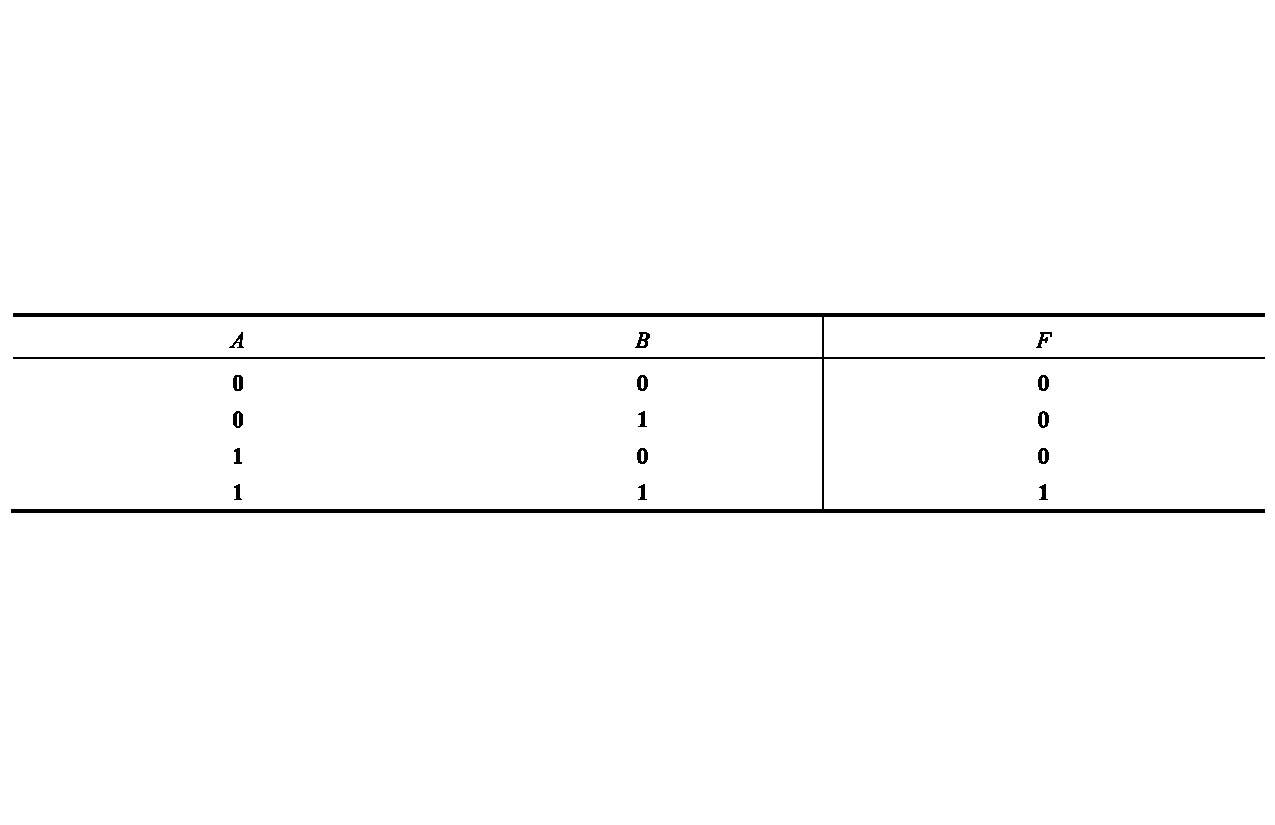
\includegraphics[width=0.98\textwidth]{与运算真值表.pdf}
        \label{tbl:与运算真值表}
    \end{table}

    \begin{wrapfigure}[5]{r}{0.25\textwidth}
        \centering
        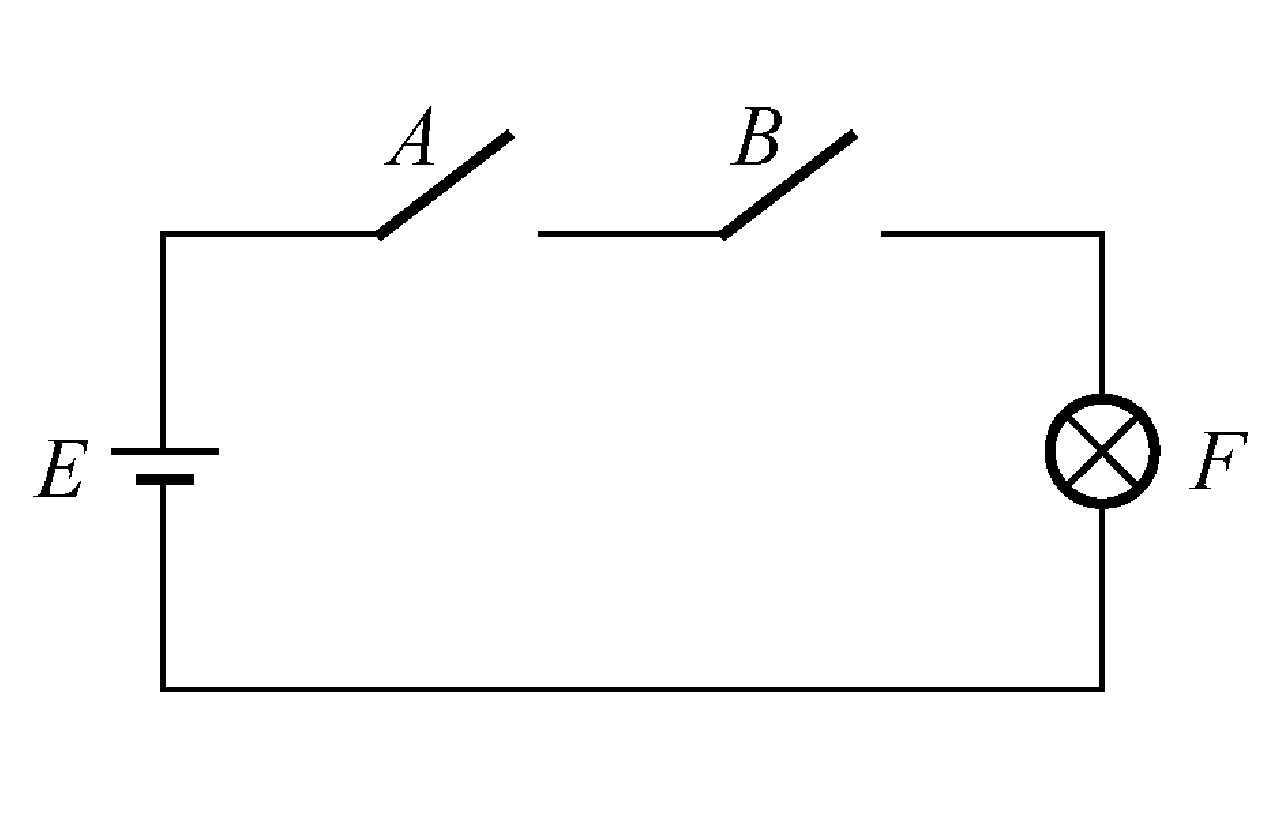
\includegraphics[width=0.25\textwidth]{与门演示电路.pdf}
        \caption{与门演示电路}
        \label{fig:与门演示电路}
    \end{wrapfigure}
    \Par 一般我们将它的电路表示成图\ref{fig:与门演示电路}中的样子,同时,我们一般用图\ref{fig:与门实现电路}中的电路来实现与门.我们约定,高电位(高电平)代表信号“真”,低电位(低电平)代表信号“假”.高电位一般取2.4V$\sim$5V,其经典值为3.6V;低电位一般取0$\sim$0.4V,其经典值为0.3V.

    \Par 当A、B两端接入低电位,即真值表的第1行,这样两个二极管导通,5V的电压降全在电阻R上,输出端F的电位与A、B相同,为低电位.

    \Par 当A、B两端一个接入高电位,一个接入低电位,即真值表的第2、3行,不妨设A接入高电位,B接入低电位.这样如果A导通,B截止,那么此时F输出端就会在高电位,此时B二极管就会被导通,使F输出端恢复低电位.

    \Par 当A、B两端接入高电位,即真值表的第4行,这样两个二极管导通,输出端F的电位与A、B相同,为高电位.
    \begin{figure}[htbp]
        \centering
        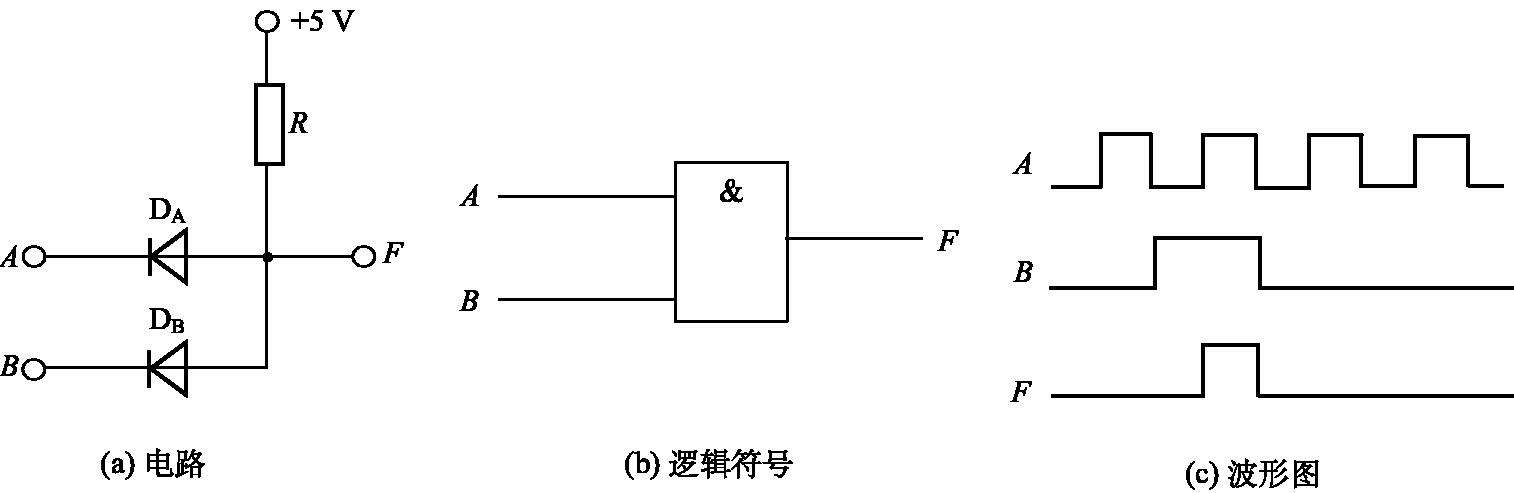
\includegraphics[width=0.85\textwidth]{与门实现电路.jpg}
        \caption{与门实现电路}
        \label{fig:与门实现电路}
    \end{figure}

    \circledtext{2}\textbf{或门}$\boldsymbol{A}+\boldsymbol{B}$

    \Par 或门的真值表如表\ref{tbl:与运算真值表}所示,与运算(逻辑乘)表示这样一种逻辑关系:在决定一件事情发生的所有条件中,只要有一个条件具备,这件事就会发生.

    \begin{table}[htbp]
        \centering
        \caption{或运算真值表}
        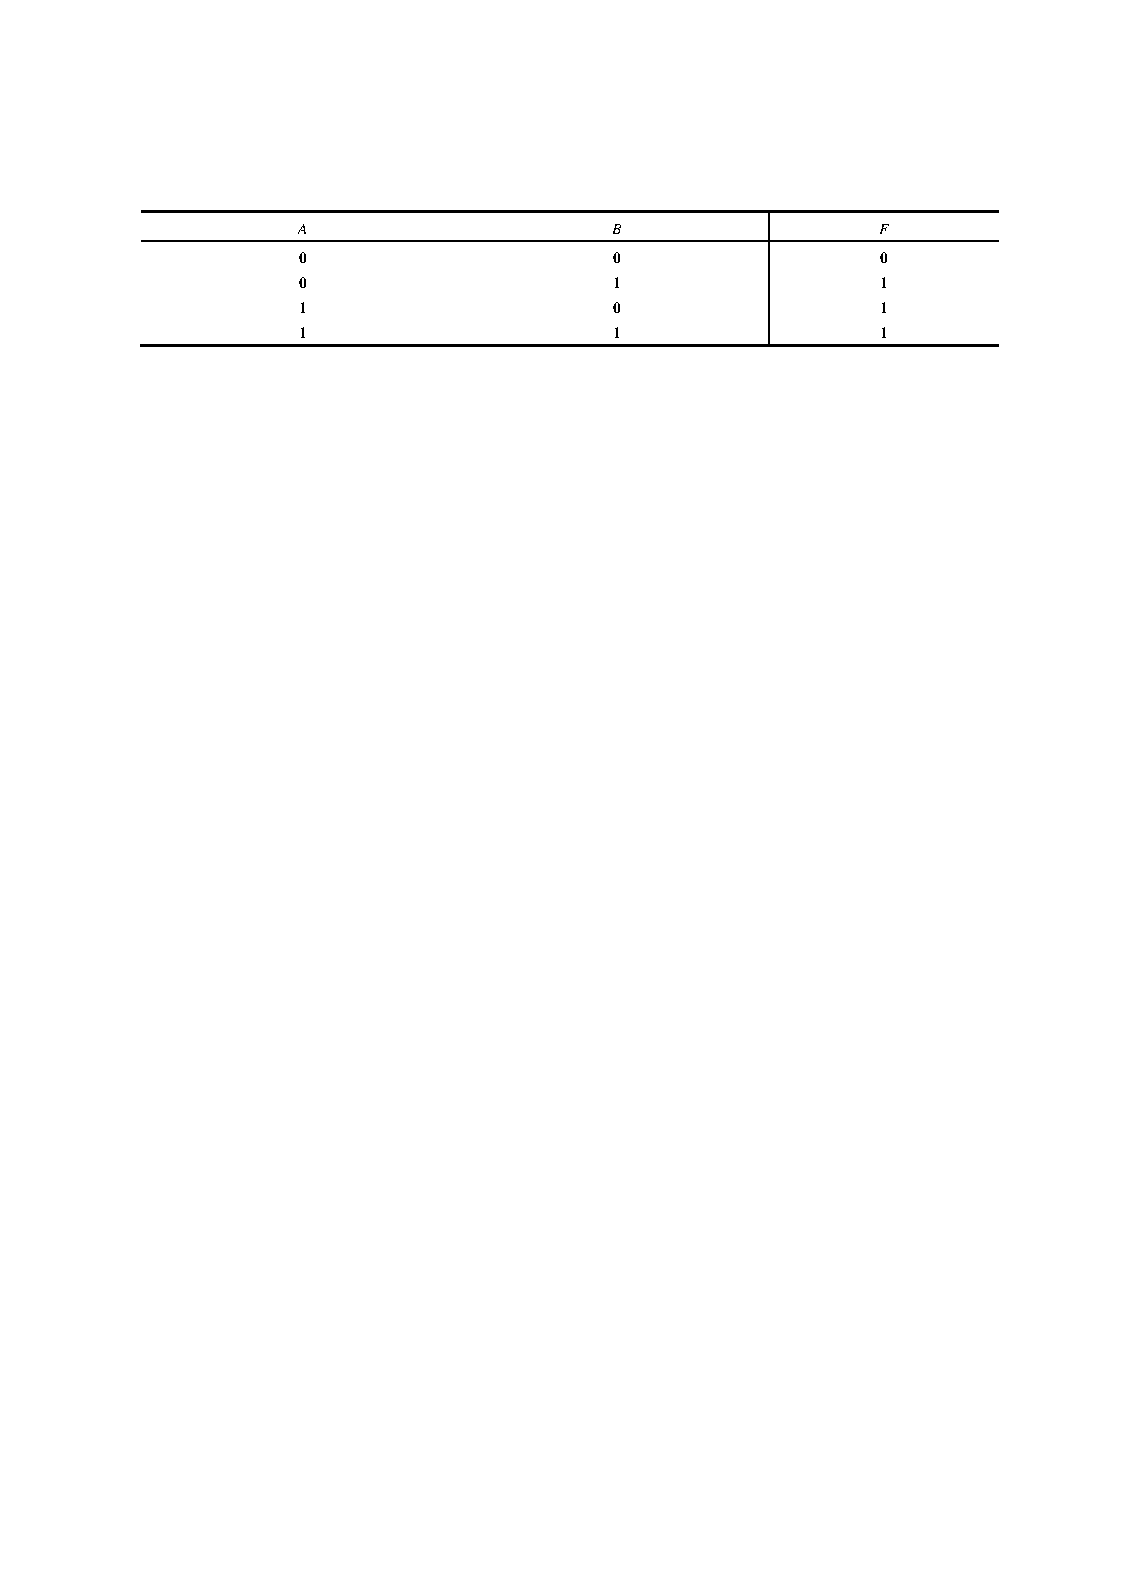
\includegraphics[width=0.98\textwidth]{或运算真值表.pdf}
        \label{tbl:或运算真值表}
    \end{table}
    
    \begin{wrapfigure}[6]{r}{0.25\textwidth}
        \centering
        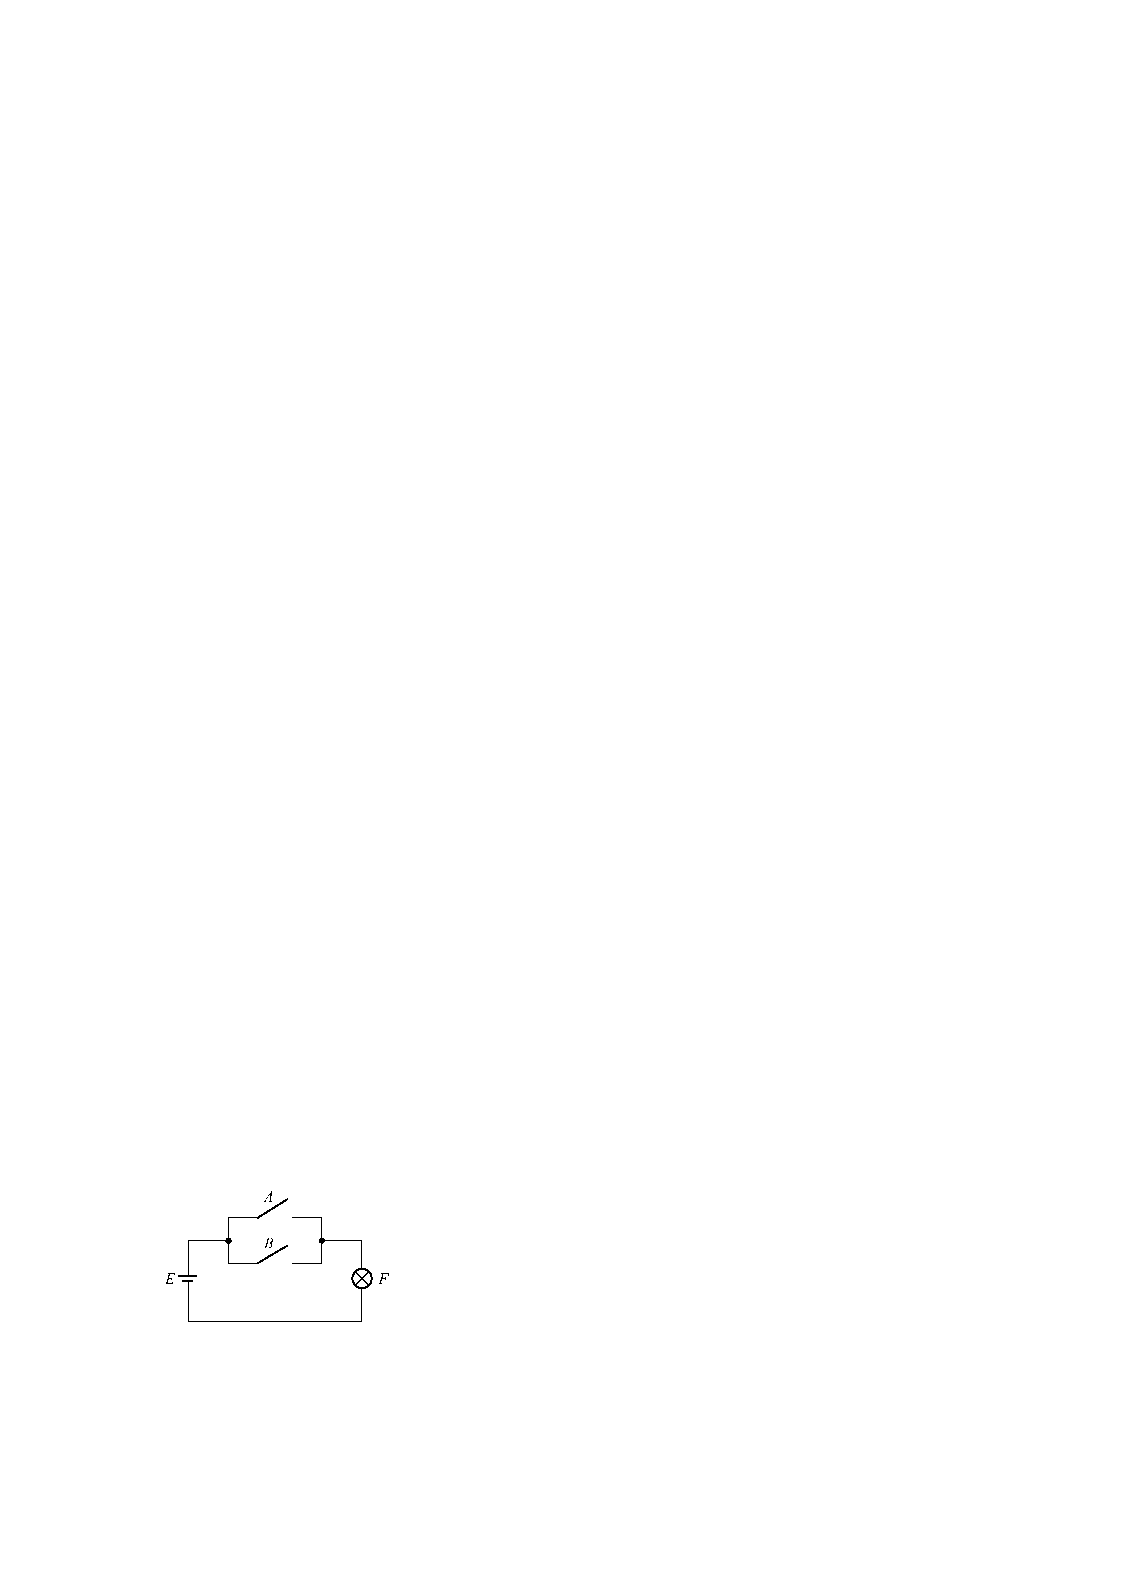
\includegraphics[width=0.25\textwidth]{或门演示电路.pdf}
        \caption{或门演示电路}
        \label{fig:或门演示电路}
    \end{wrapfigure}
    \Par 一般我们将它的电路表示成图\ref{fig:或门演示电路}中的样子,同时,我们一般用图\ref{fig:或门实现电路}中的电路来实现或门.
    
    \Par 当A、B两端接入低电位,即真值表的第1行,此时无论二极管导不导通,输出端F的电位都是低电位.
    
    \Par 当A、B两端一个接入高电位,一个接入低电位,即真值表的第2、3行,不妨设A接入高电位,B接入低电位.如果二极管B导通,那么二极管左端电位高,右端电位低,它就会导通使得二极管B截止,此时输出端F电位与A相同是高电位.
    
    \Par 当A、B两端接入高电位,即真值表的第4行,此时二极管A、B均导通输出端F电位与A、B相同是高电位.
    \begin{figure}[htbp]
        \centering
        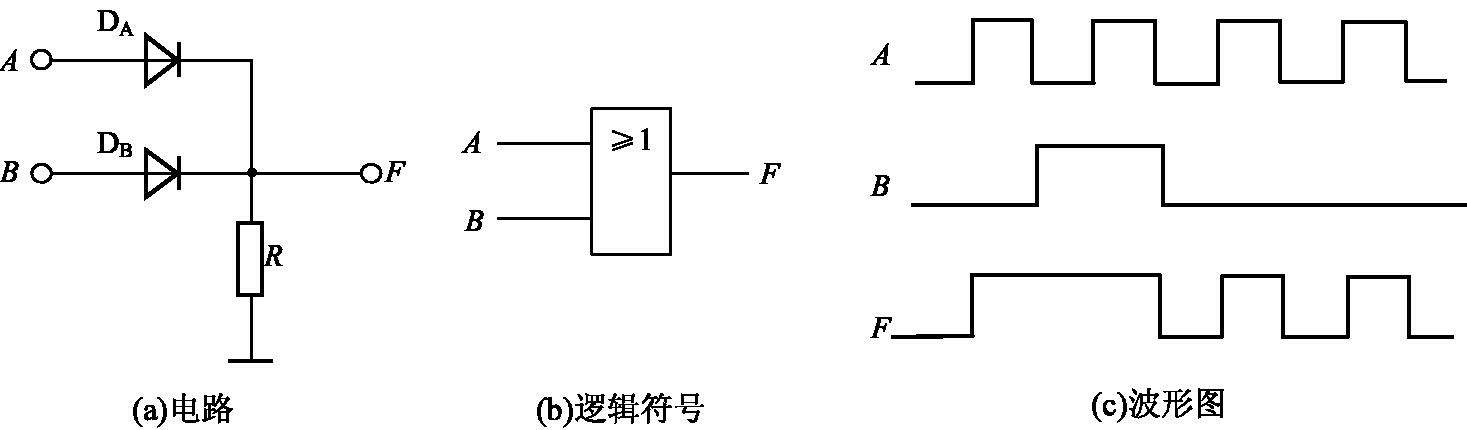
\includegraphics[width=0.85\textwidth]{或门实现电路.jpg}
        \caption{或门实现电路}
        \label{fig:或门实现电路}
    \end{figure}


    \circledtext{3}\textbf{非门}$\overline{\boldsymbol{A}}$

    \begin{wrapfigure}{r}{0.25\textwidth}
        \centering
        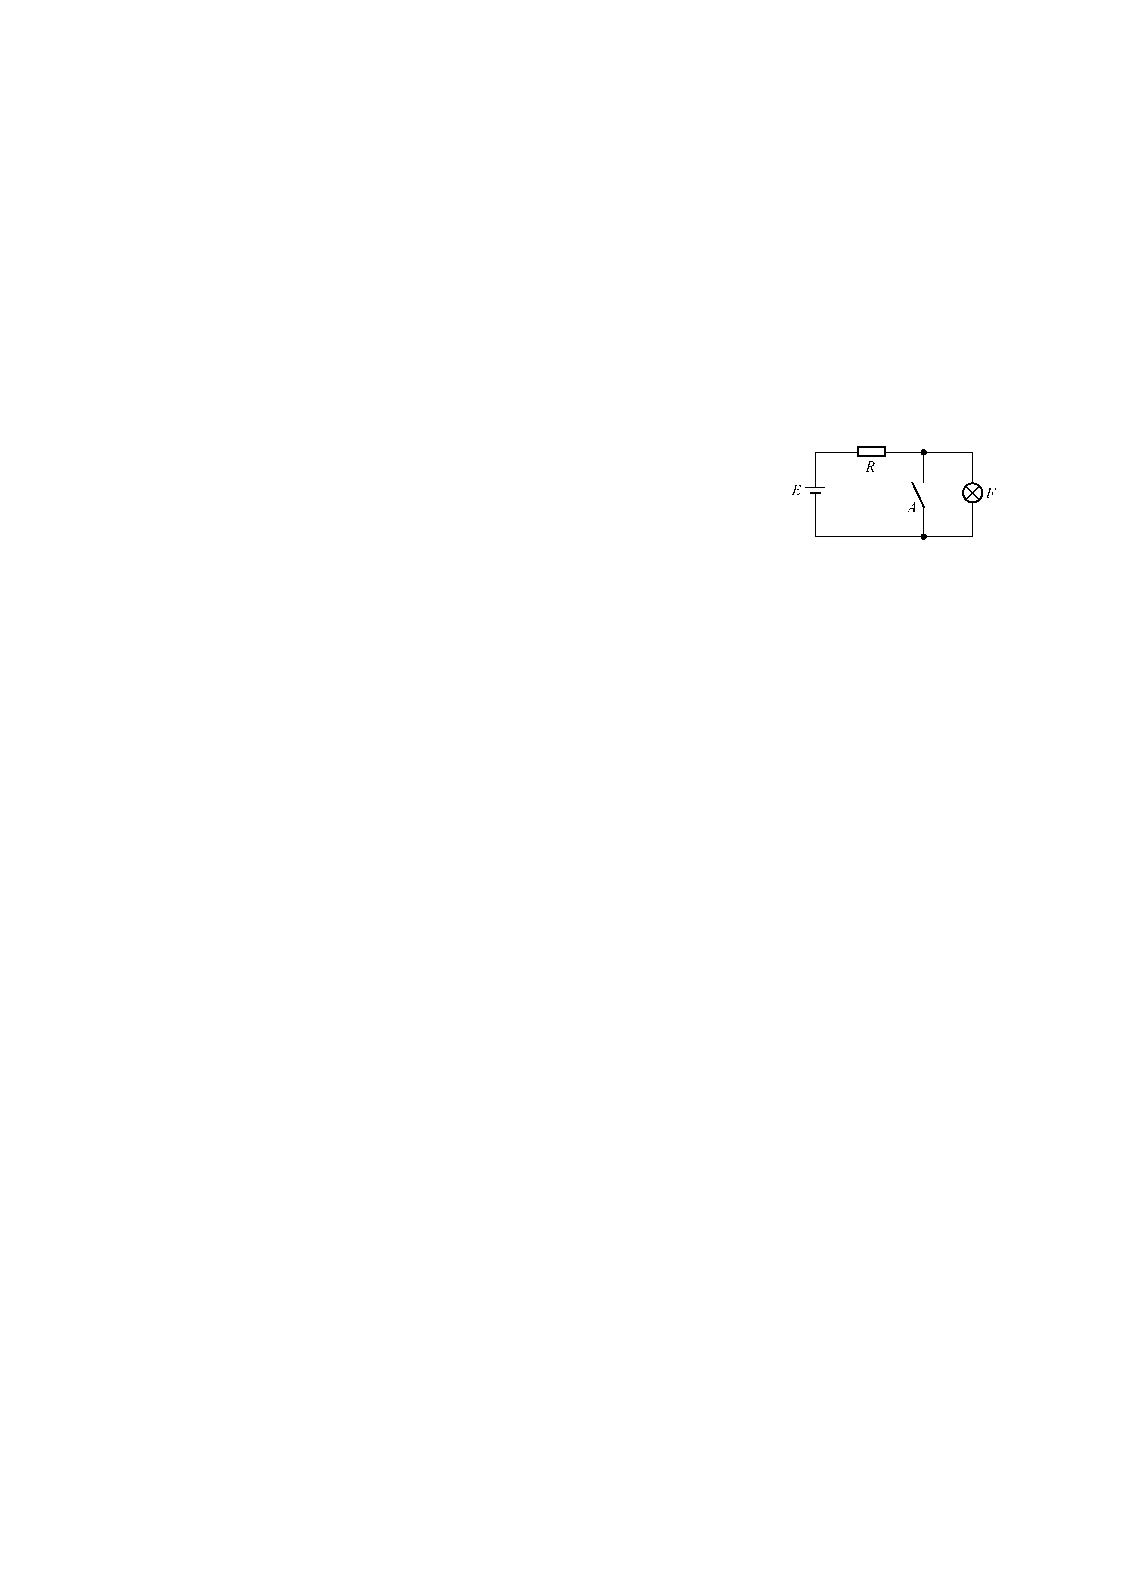
\includegraphics[width=0.25\textwidth]{非门演示电路.pdf}
        \caption{非门演示电路}
        \label{fig:非门演示电路}
    \end{wrapfigure}
    \Par 非门的真值表如表\ref{tbl:与运算真值表}所示,与运算(逻辑乘)表示这样一种逻辑关系:当条件具备时,结果不会发生;当条件不具备时,结果一定会发生.

    \begin{table}[htbp]
        \centering
        \caption{非运算真值表}
        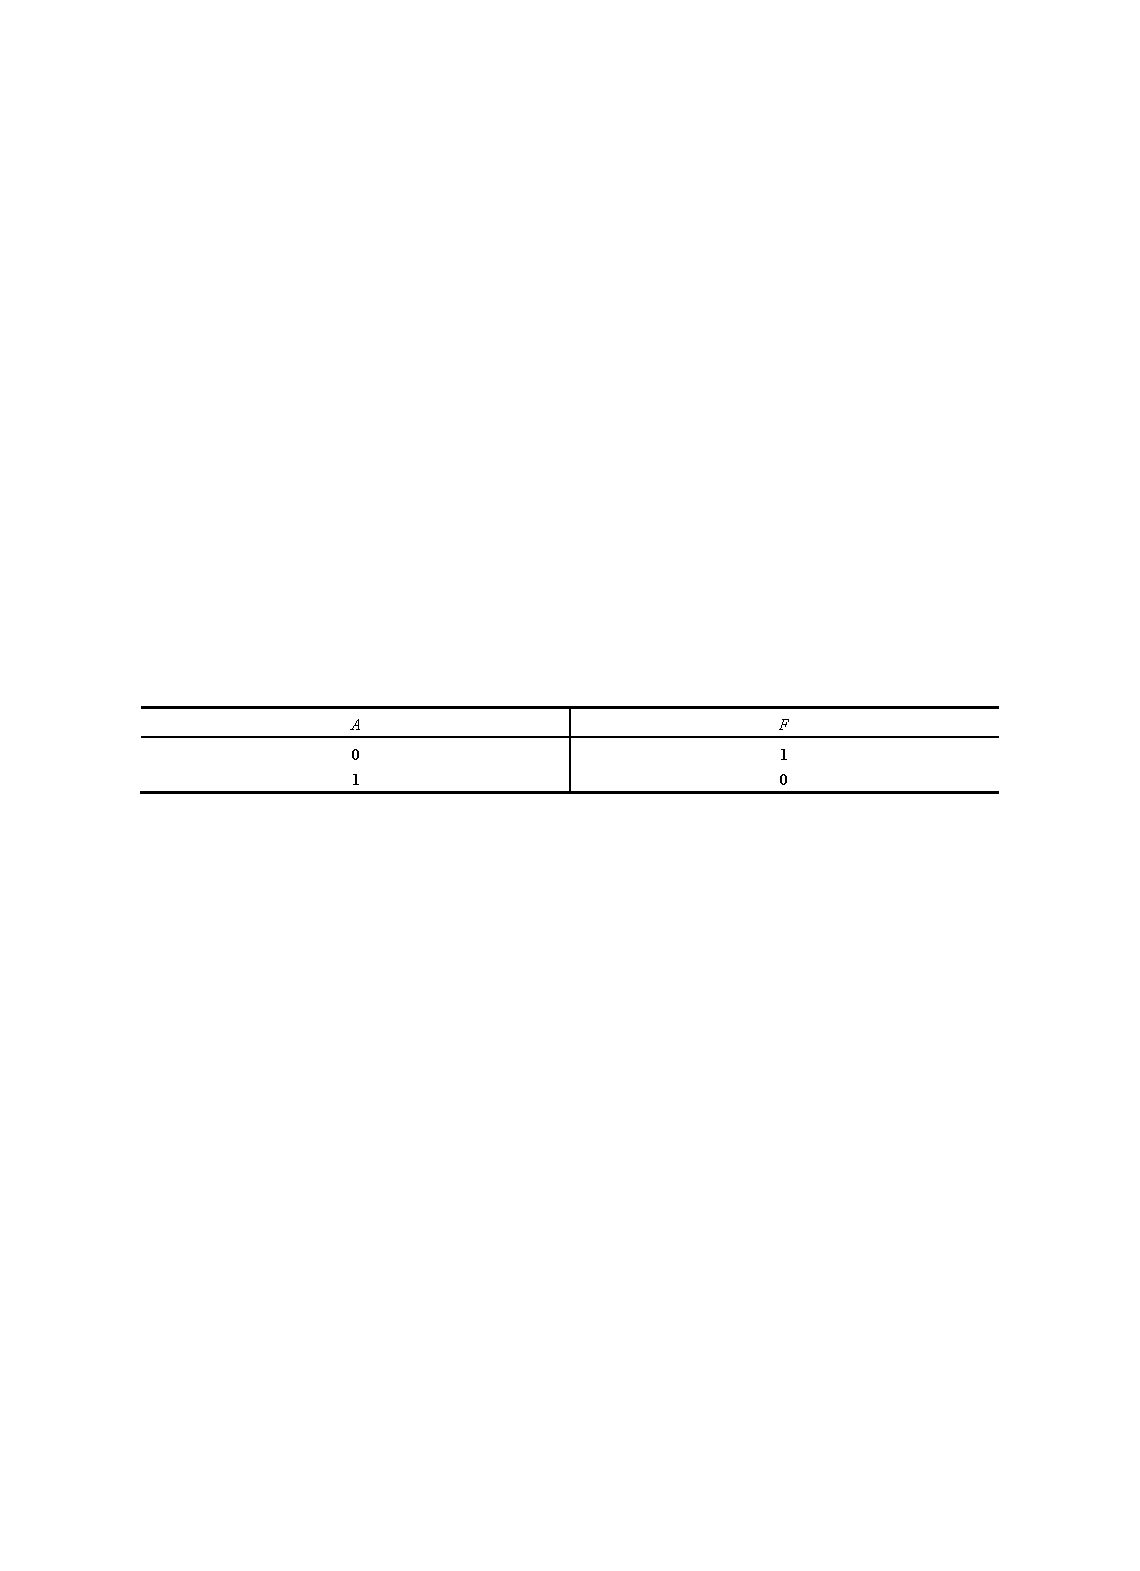
\includegraphics[width=0.98\textwidth]{非运算真值表.pdf}
        \label{tbl:非运算真值表}
    \end{table}
    
    
    \Par 一般我们将它的电路表示成图\ref{fig:非门演示电路}中的样子,同时,我们一般用图\ref{fig:非门实现电路}中的电路来实现非门.
    
    \begin{figure}[htbp]
        \centering
        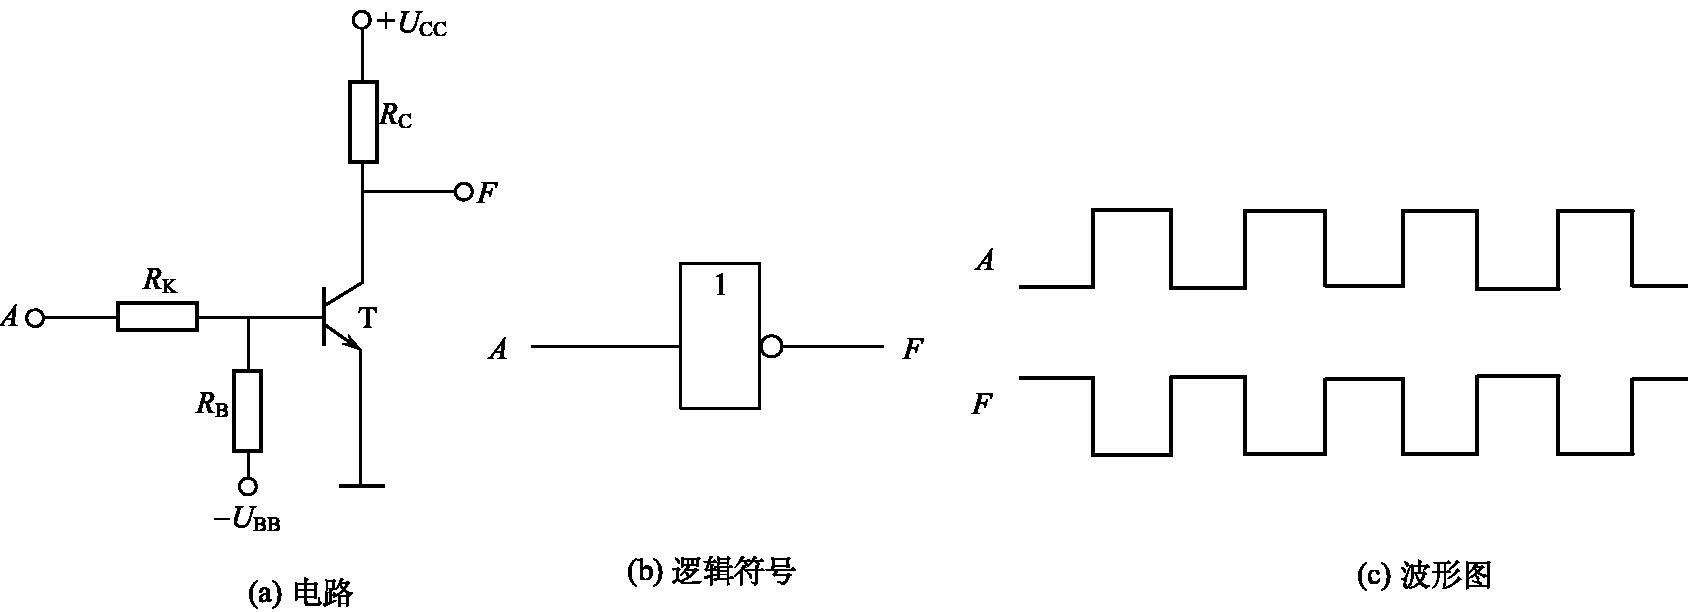
\includegraphics[width=0.85\textwidth]{非门实现电路.jpg}
        \caption{非门实现电路}
        \label{fig:非门实现电路}
    \end{figure}

    与非
    \begin{equation}
        \overline{\boldsymbol{A}\cdot \boldsymbol{B}}
    \end{equation}

    或非
    \begin{equation}
        \overline{\boldsymbol{A}+\boldsymbol{B}}
    \end{equation}

    与或非
    \begin{equation}
        \overline{\boldsymbol{A}\cdot \boldsymbol{B}+\boldsymbol{C}\cdot \boldsymbol{D}}
    \end{equation}

    异或
    \begin{equation}
        \boldsymbol{F}=\boldsymbol{A}\oplus \boldsymbol{B}=\overline{\boldsymbol{A}}\cdot \boldsymbol{B}+\boldsymbol{A}\cdot \overline{\boldsymbol{B}}
    \end{equation}

    \begin{table}[htbp]
        \centering
        \caption{异或运算真值表} 
        \label{fig:异或运算真值表}
        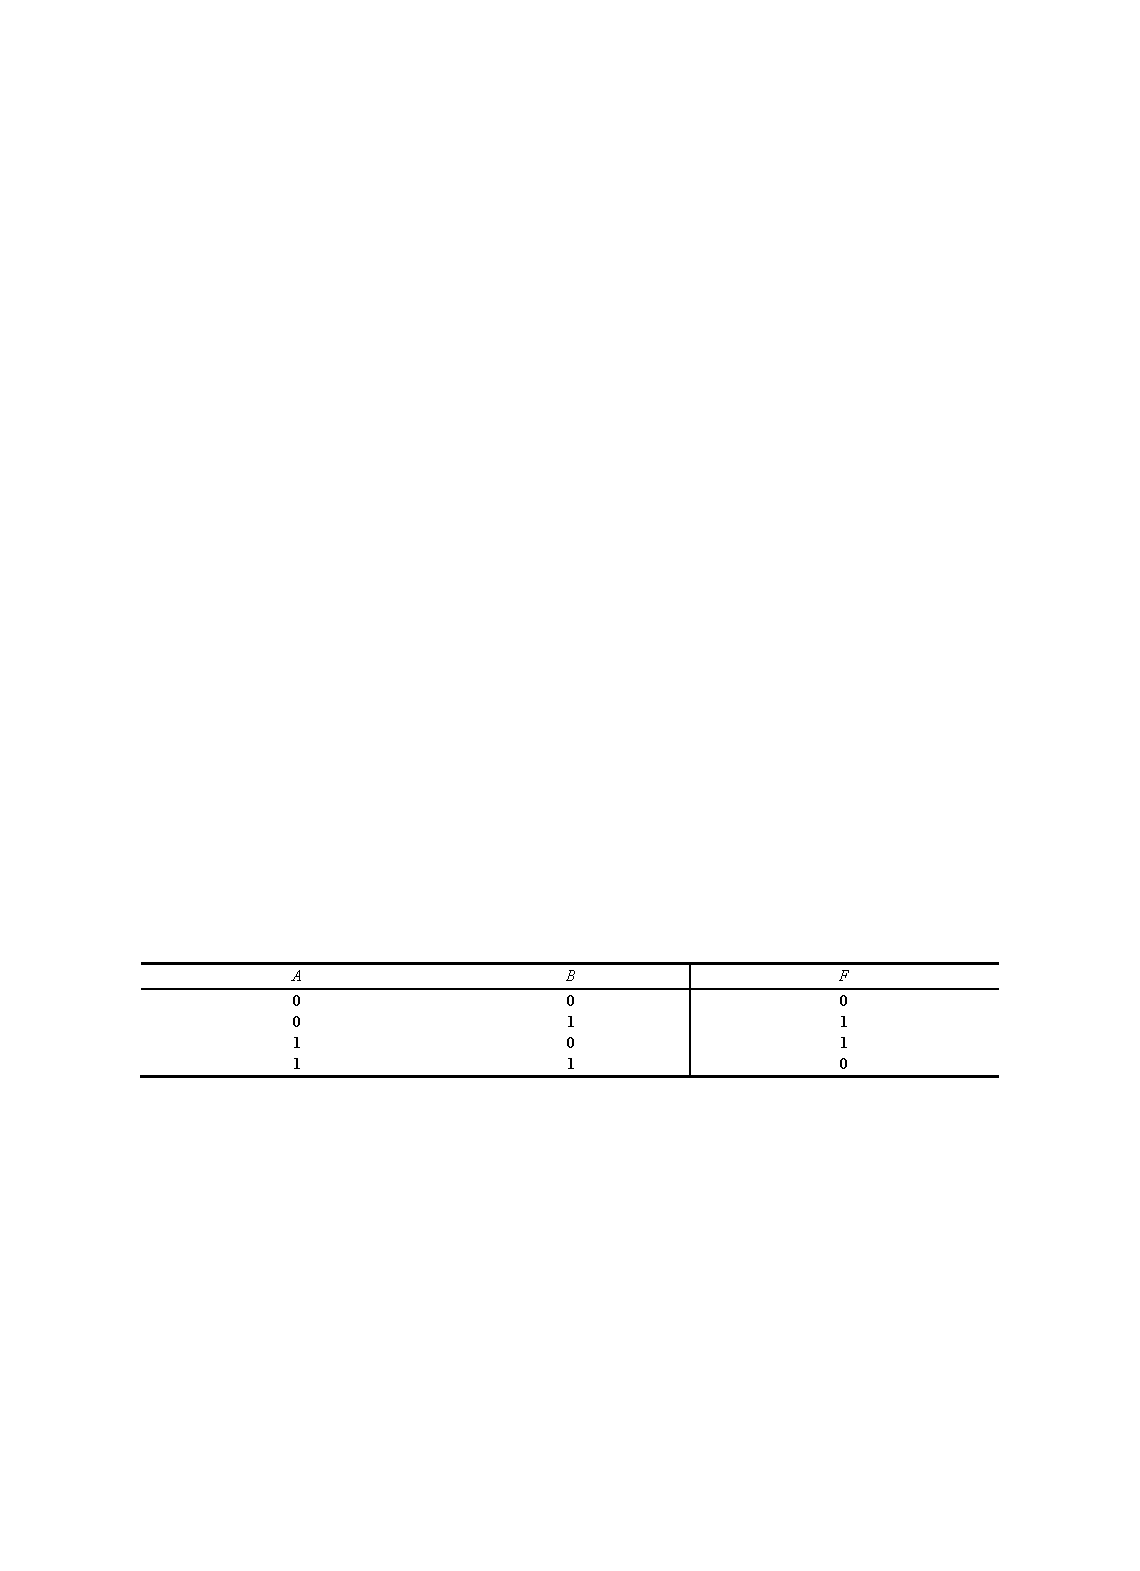
\includegraphics[width=0.95\textwidth]{异或运算真值表.pdf}
         
    \end{table}

    同或
    \begin{equation}
        \boldsymbol{F}=\boldsymbol{A}\odot \boldsymbol{B}=\boldsymbol{A}\cdot \boldsymbol{B}+\overline{\boldsymbol{A}}\cdot \overline{\boldsymbol{B}}
    \end{equation}

    \begin{table}[htbp]
        \centering
        \caption{同或运算真值表}
        \label{fig:同或运算真值表}
        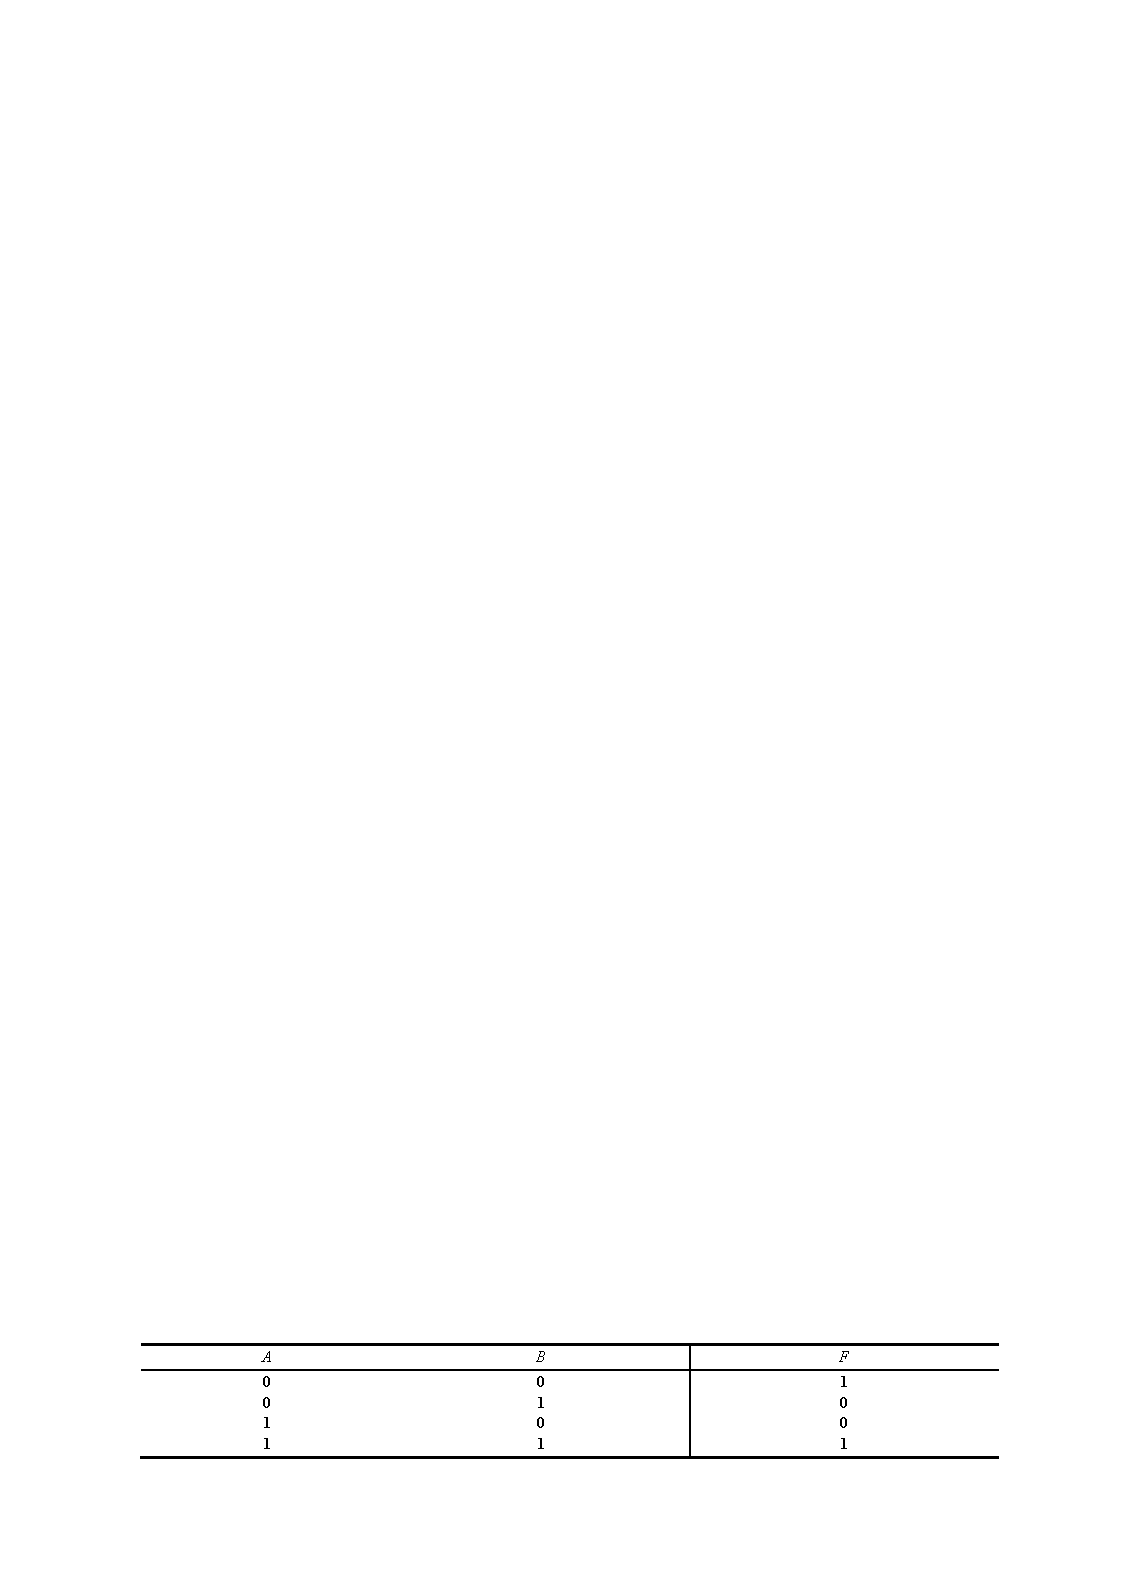
\includegraphics[width=0.95\textwidth]{同或运算真值表.pdf}
          
    \end{table}

    从真值表我们就可以看出,异或逻辑与同或逻辑互为反函数,即
    \begin{equation}
        \overline{\boldsymbol{A}\oplus \boldsymbol{B}}=\boldsymbol{A}\odot \boldsymbol{B}\Longleftrightarrow \boldsymbol{A}\oplus \boldsymbol{B}=\overline{\boldsymbol{A}\odot \boldsymbol{B}}
    \end{equation}



\section{\K 逻辑代数}
\Par 我们先给出基础的9条规则
\begin{equation*}
    \begin{matrix}
        \begin{aligned}
        \boldsymbol{A}\cdot 1&=\boldsymbol{A}\\
        \boldsymbol{A}\cdot 0&=0\\
        \boldsymbol{A}\cdot \boldsymbol{A}&=\boldsymbol{A}\\
        \boldsymbol{A}\cdot \overline{\boldsymbol{A}}&=0\\
    \end{aligned}&		\begin{aligned}
        \boldsymbol{A}+1&=1\\
        \boldsymbol{A}+0&=\boldsymbol{A}\\
        \boldsymbol{A}+\boldsymbol{A}&=\boldsymbol{A}\\
        \boldsymbol{A}+\overline{\boldsymbol{A}}&=1\\
    \end{aligned}&		\begin{array}{c}
        \overline{\overline{\boldsymbol{A}}}=\boldsymbol{A}\\
        \\
        \\
        \\
    \end{array}\\
    \end{matrix}
\end{equation*}

然后需要指出,不同于普通运算,逻辑代数的与运算和或运算具有同等优先级,这体现在交换律

\textbf{交换律}
\begin{align}
	\boldsymbol{A}\cdot \left( \boldsymbol{B}+\boldsymbol{C} \right) &=\left( \boldsymbol{A}\cdot \boldsymbol{B} \right) +\left( \boldsymbol{A}\cdot \boldsymbol{C} \right)\\
	\boldsymbol{A}+\left( \boldsymbol{B}\cdot \boldsymbol{C} \right) &=\left( \boldsymbol{A}+\boldsymbol{B} \right) \cdot \left( \boldsymbol{A}+\boldsymbol{C} \right)
\end{align}

\textbf{结合律}
\begin{align}
	\boldsymbol{A}\cdot \boldsymbol{B}\cdot \boldsymbol{C}&=\left( \boldsymbol{A}\cdot \boldsymbol{B} \right) \cdot \boldsymbol{C}=\boldsymbol{A}\cdot \left( \boldsymbol{B}\cdot \boldsymbol{C} \right)\\
	\boldsymbol{A}+\boldsymbol{B}+\boldsymbol{C}&=\left( \boldsymbol{A}+\boldsymbol{B} \right) +\boldsymbol{C}=\boldsymbol{A}+\left( \boldsymbol{B}+\boldsymbol{C} \right)
\end{align}

\textbf{交换律}
\begin{align}
	\boldsymbol{A}+\boldsymbol{B}&=\boldsymbol{B}+\boldsymbol{A}\\
	\boldsymbol{A}\cdot \boldsymbol{B}&=\boldsymbol{B}\cdot \boldsymbol{A}
\end{align}

\textbf{反演律}
\begin{align}
	\overline{\boldsymbol{A}\cdot \boldsymbol{B}}&=\overline{\boldsymbol{A}}+\overline{\boldsymbol{B}}\\
	\overline{\boldsymbol{A}+\boldsymbol{B}}&=\overline{\boldsymbol{A}}\cdot \overline{\boldsymbol{B}}
\end{align}

另有一些常用的公式:

\textbf{合并律}